\begin{frame}{Definition of Efficiency Metrics}
    \textbf{In General}
	\begin{itemize}
        \item One Track Event $\implies$ NOT reconstructed
        \item Two Track event + Opposite charges $\implies$ reconstructed 
        \item More than two track $\implies$ complicated
    \end{itemize}
    \vspace{1 cm}
    \textbf{Some Possible Eff. Metrics}
    \begin{itemize}
        \item Number of Events with $\geq$ 2 longTracks [good proxy]
        \item (Can add charge identification to above but not necessary)
        \item MC Based Effi. [matching reconstructed to truth level data]
    \end{itemize}
\end{frame}

\begin{frame}{Definition of Fiducial}
    Before we define the efficiency we need to account for the detector acceptance by requiring the particle to be Fiducial.

		\textbf{Based on reconstructed data [Adapted from Sinead]}
		\begin{itemize}
			\item Requires $longTracks == 2$ 
			\item $Track\_r\_atMaxRadius < 100$
			\item $t\_st\{1,2,3\}\_r < 100$
 		\end{itemize}
		\textbf{Based on truth level data }
		\begin{itemize}
			\item $truthd0\_r [\{1,2,3\}] < 100$
			\item $truthd1\_r [\{1,2,3\}] < 100$
			\item Does not need the 2track cut while maintaining that particles of interest were Fiducial, While also being independent of ALMA9 or CENTOS7
	
		\end{itemize}

        \textbf{Note:}
        \begin{itemize}
		\item Where are NaNs coming from at the truth-level?
	    \end{itemize}	
\end{frame}

\begin{frame}{How do Fiducial Cuts perform?}
    \begin{table}[h!]
        \centering
        \small
        \begin{tabular}{|l|c|c|c|c|}
        \hline
        \textbf{Selection Step} & \textbf{Pass} & \textbf{All} & \textbf{Effi. (\%)} & \textbf{Cum. Effi. (\%)} \\ \hline
        2LongTracks              & 37807        & 60000       & 63.01                   & 63.01                              \\ \hline
        Opposite Charge          & 32427        & 37807       & 85.77                   & 54.04                              \\ \hline
        MaxRadius $<$ 100        & 31489    & 32427       & 97.11                   & 52.48                              \\ \hline
        $t\_st1\_r < 100$        & 31471        & 31489       & 99.94                   & 52.45                              \\ \hline
        $t\_st2\_r < 100$        & 31458        & 31471       & 99.96                   & 52.43                              \\ \hline
        $t\_st3\_r < 100$        & 31383        & 31458       & 99.76                   & 52.31                              \\ \hline
        \end{tabular}
        \caption{Efficiencies and cumulative efficiencies at various selection steps. [ALMA9]}
        \label{table:efficiency}
    \end{table}
    \vspace{-0.5cm}
    \begin{table}[h!]
        \centering
        \small
        \begin{tabular}{|l|c|c|c|c|}
        \hline
        \textbf{Selection Step} & \textbf{Pass} & \textbf{All} & \textbf{Effi. (\%)} & \textbf{Cum. Effi. (\%)} \\ \hline
        2LongTracks              & 36746        & 60000       & 61.24                   & 61.24                              \\ \hline
        Opposite Charge          & 30375        & 36746       & 82.66                   & 50.62                              \\ \hline
        MaxRadius $<$ 100 & 29520    & 30375       & 97.19                   & 49.20                              \\ \hline
        $t\_st1\_r < 100$        & 29498        & 29520       & 99.93                   & 49.16                              \\ \hline
        $t\_st2\_r < 100$        & 29491        & 29498       & 99.98                   & 49.15                              \\ \hline
        $t\_st3\_r < 100$        & 29415        & 29491       & 99.74                   & 49.03                              \\ \hline
        \end{tabular}
        \caption{Efficiencies and cumulative efficiencies at various selection steps.[CENTOS7]}
        \label{table:efficiency_updated}
        \end{table}        
        \vspace{-0.5cm}
        \begin{itemize}
            \item ALMA9 performs better over most of the cuts. 
            \item Using this fiducial cuts throws out 50\% of the data.
        \end{itemize}        
\end{frame}

\begin{frame}{Cuts. Contd.}
    \begin{table}[h!]
        \centering
        \small
        \begin{tabular}{|l|c|c|c|c|}
        \hline
        \textbf{Selection Step} & \textbf{Pass} & \textbf{All} & \textbf{Effi. (\%)} & \textbf{Cum. Effi. (\%)} \\ \hline
        truthd\{0,1\}\_st1\_r $<$ 100    & 59634        & 60000       & 99.39                   & 99.39                              \\ \hline
        truthd\{0,1\}\_st2\_r $<$ 100   & 58429        & 59634       & 97.98                   & 97.38                              \\ \hline
        truthd\{0,1\}\_st3\_r $<$ 100   & 56703        & 58429       & 97.05                   & 94.50                              \\ \hline
        \end{tabular}
        \caption{Efficiencies and cumulative efficiencies for truth-level selection steps. [same for ALMA9/CENTOS7]}
        \label{table:truth_efficiency}
    \end{table}
        truthd\_st1\_r = \\
        \hspace{0.5cm}sqrt( pow(truthd0\_x[1],2) + pow(truthd0\_y[1],2) ) $>$ 100 \&\& \\
        \hspace{0.5cm}sqrt( pow(truthd1\_x[1],2) + pow(truthd1\_y[1],2) )
\end{frame}

\begin{frame}{Efficiency Definition}
    \begin{itemize}
        \item Remove acceptance based on fiducial cuts at truth level
        \item Define Efficiency as the fraction of events with more than 2 reconstructed longTracks divided by the total number of events. 
        \[ \text{Efficiency} = \frac{\text{NEvents}({\geq 2 \text{longTracks}})}{\text{NEvents}({\text{Total}})} \]
    \end{itemize}
\end{frame}

\begin{frame}{$>=2$ Track Efficiency as a function of DeltaR0}
    \begin{figure}
        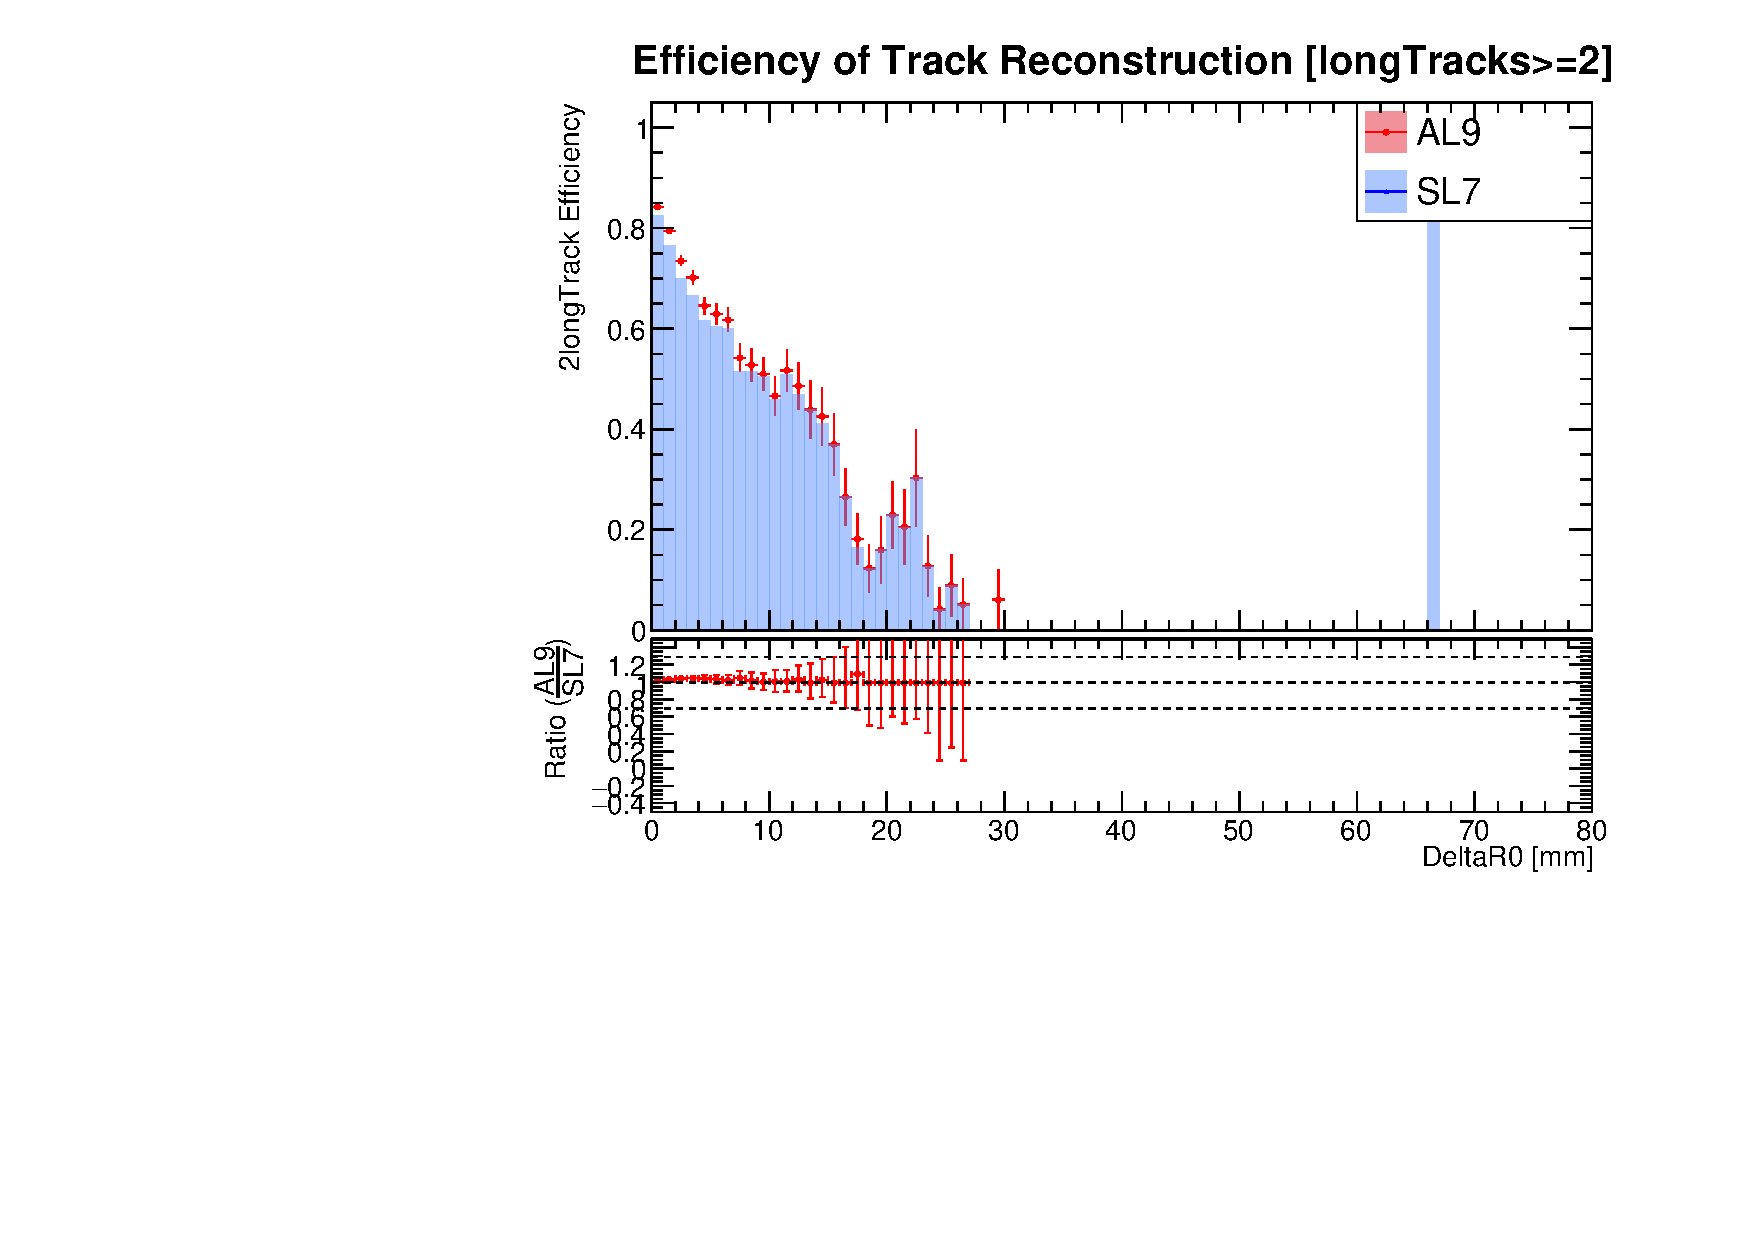
\includegraphics[width=\linewidth]{./output/Effi_greq2_DeltaR0.pdf}
    \end{figure}
\end{frame}
\begin{frame}{$>=2$ Track Efficiency as a function of DeltaX0 [SKIP]}
    \begin{figure}
        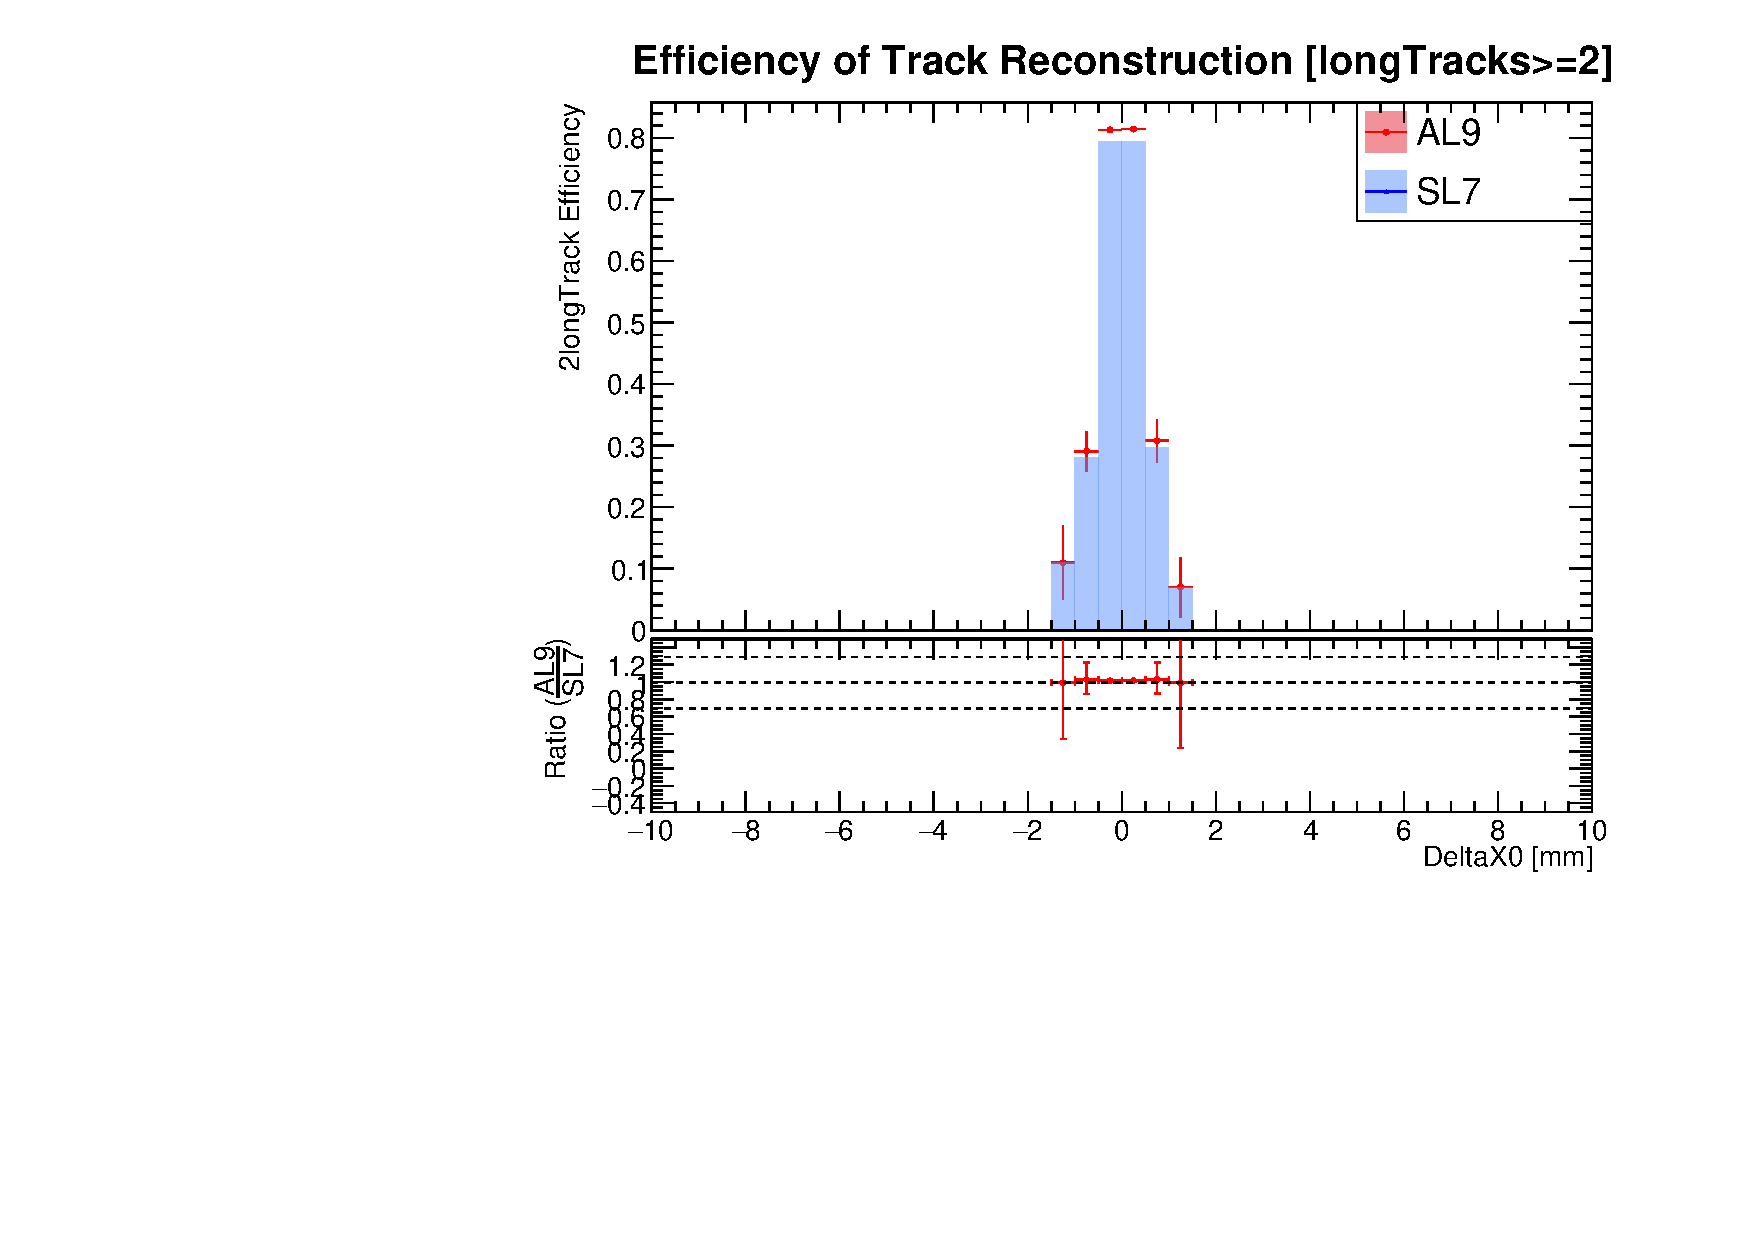
\includegraphics[width=\linewidth]{./output/Effi_greq2_DeltaX0.pdf}

    \end{figure}
\end{frame}
\begin{frame}{$>=2$ Track Efficiency as a function of DeltaY0 [SKIP]}
    \begin{figure}
        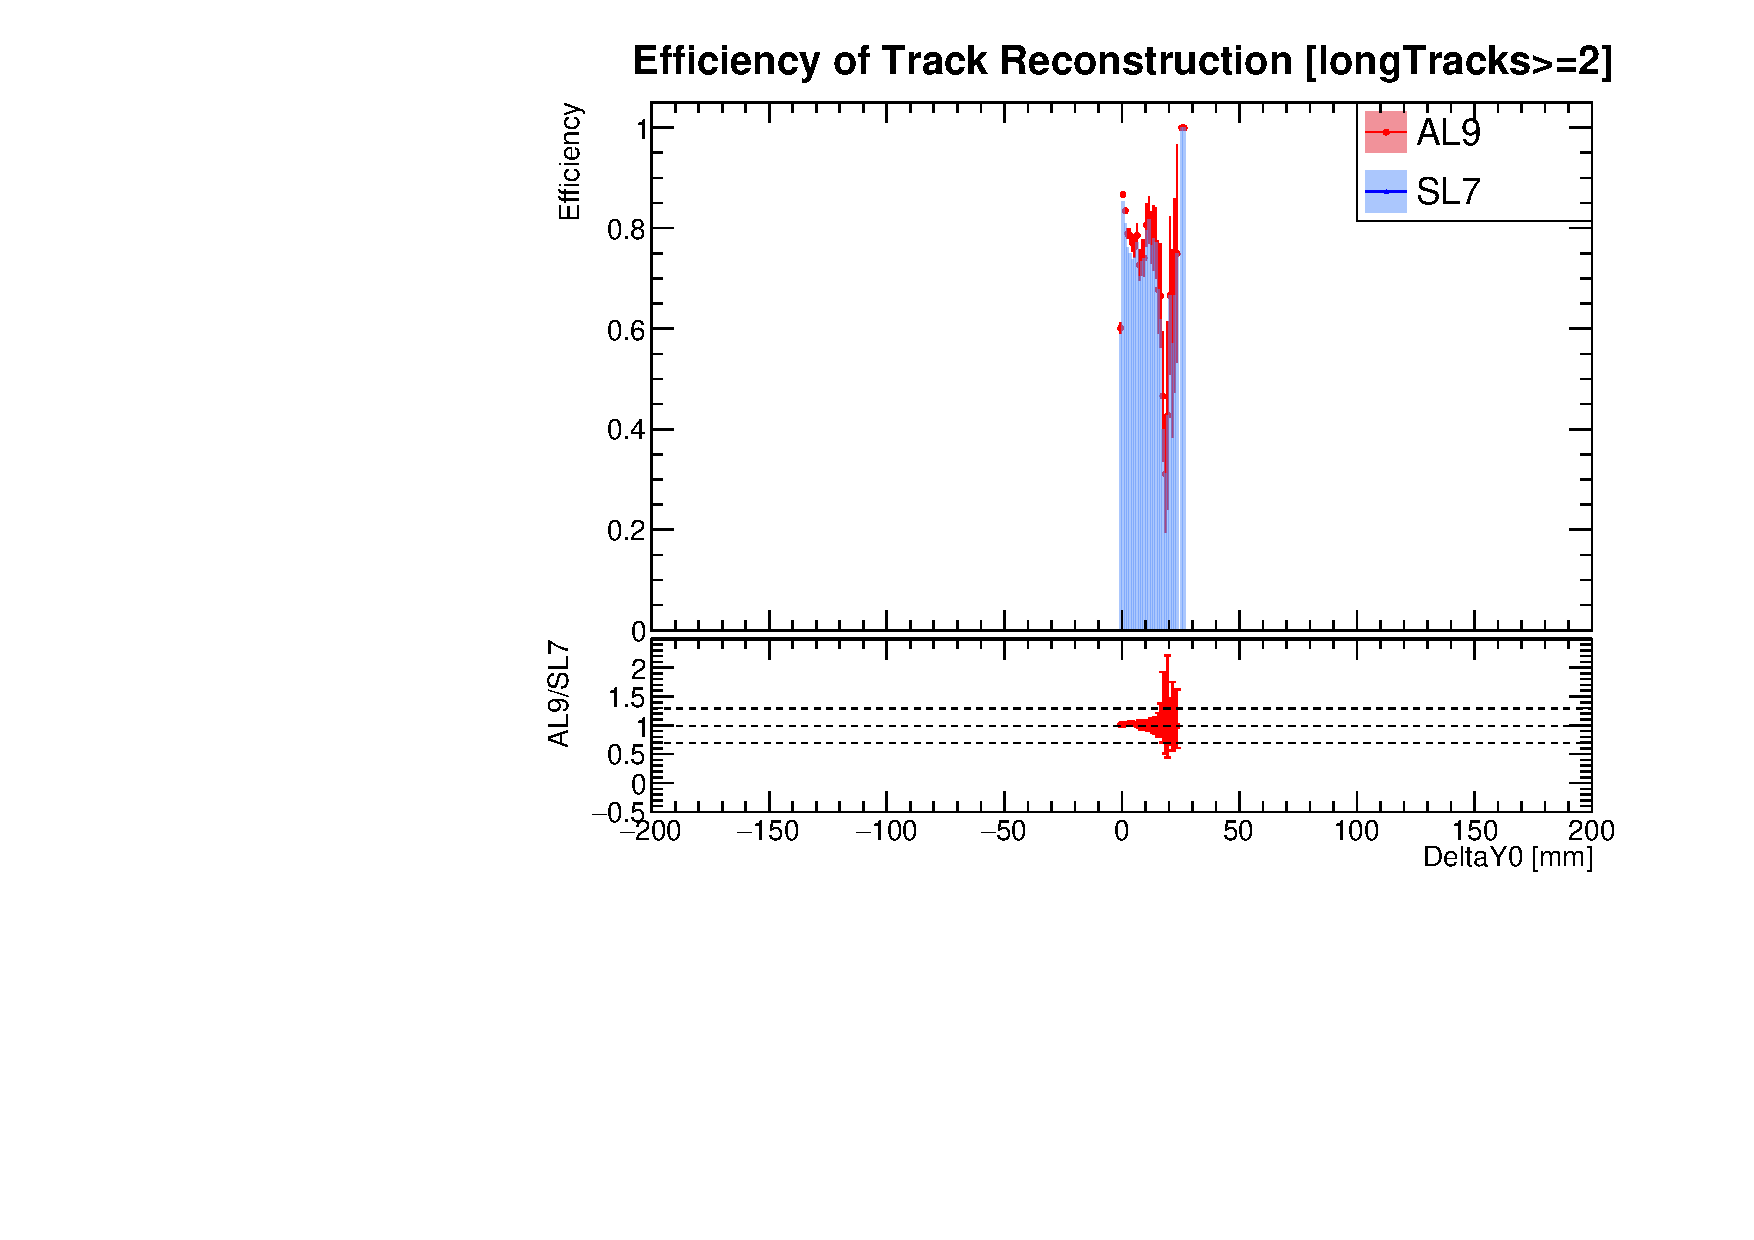
\includegraphics[width=\linewidth]{./output/Effi_greq2_DeltaY0.pdf}
    \end{figure}
\end{frame}
\begin{frame}{$>=2$ Track Efficiency as a function of Theta0}
    \begin{figure}
        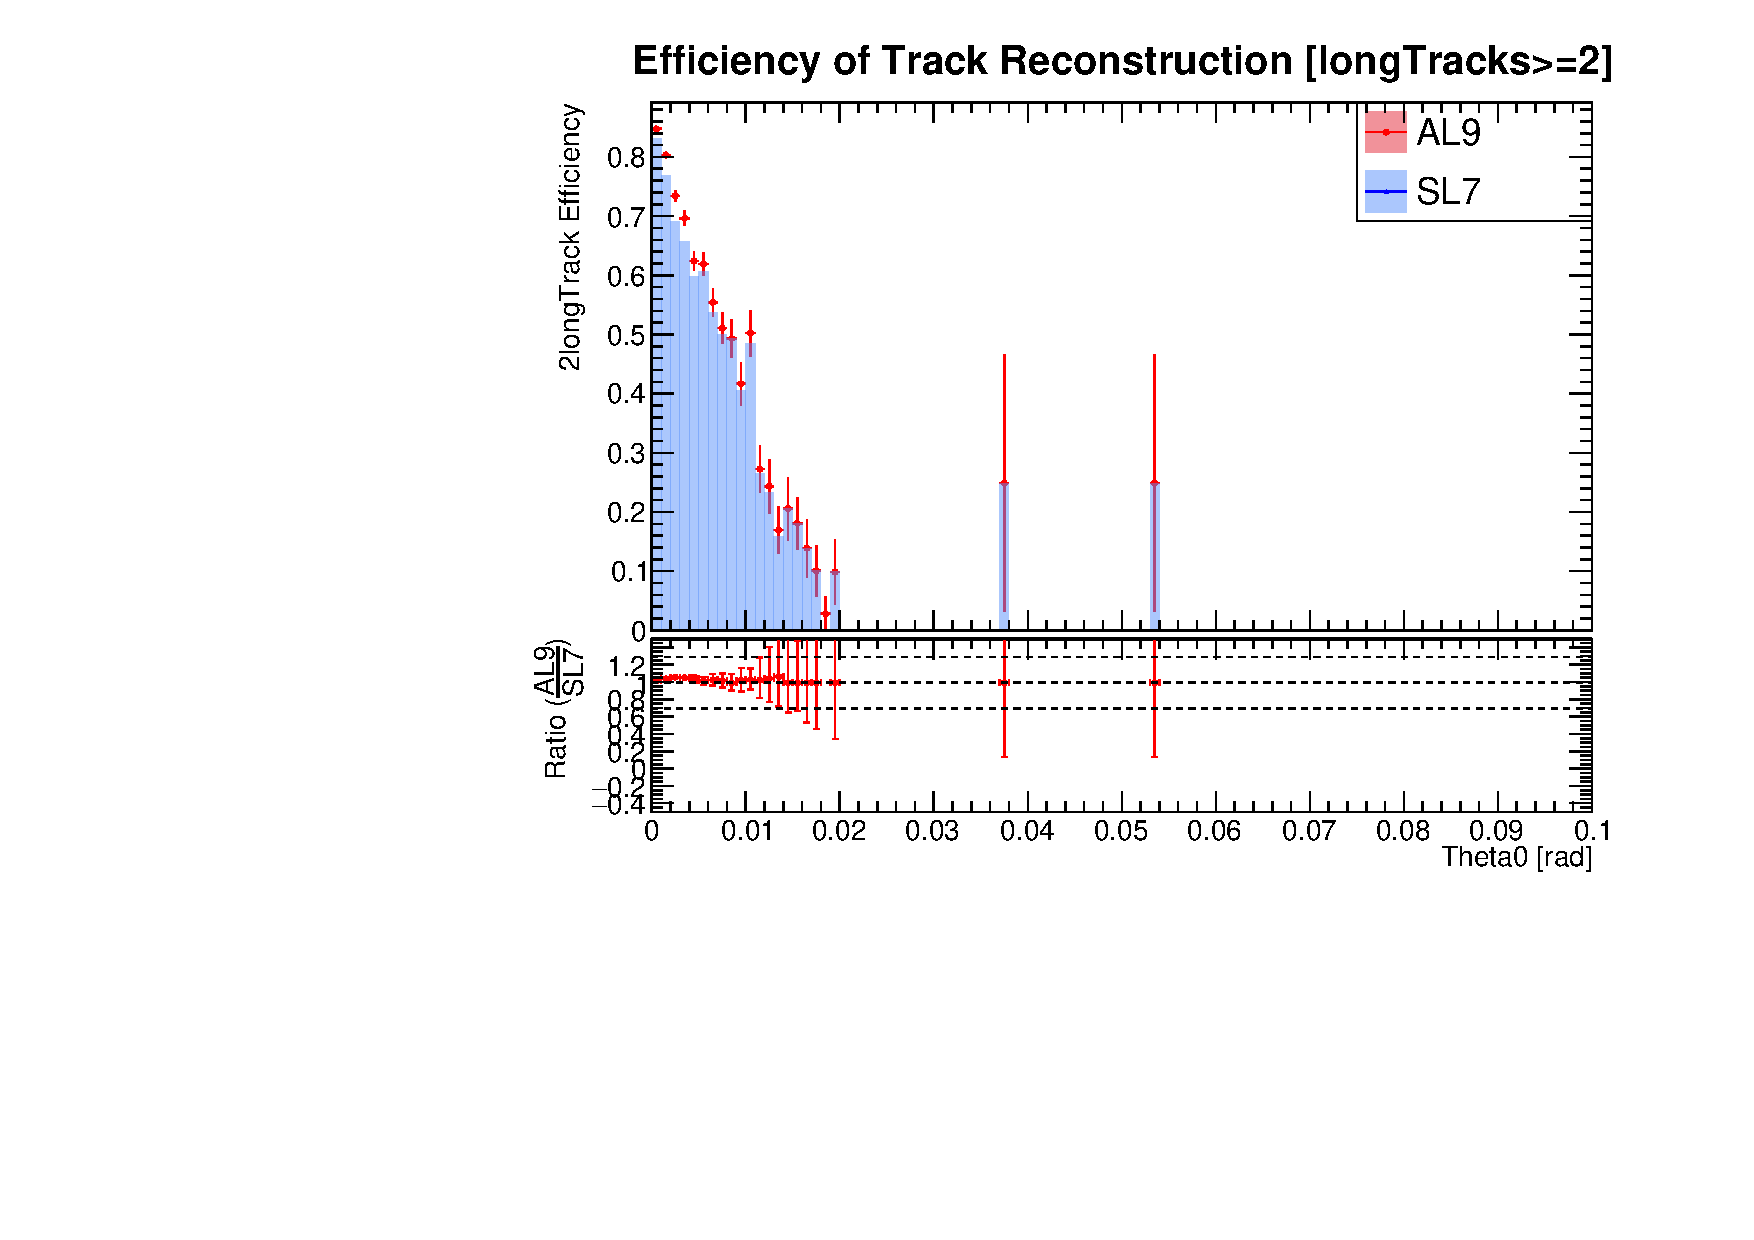
\includegraphics[width=\linewidth]{./output/Effi_greq2_Theta0.pdf}
    \end{figure}
\end{frame}
\begin{frame}{$>=2$ Track Efficiency as a function of DeltaRP}
    \begin{figure}
        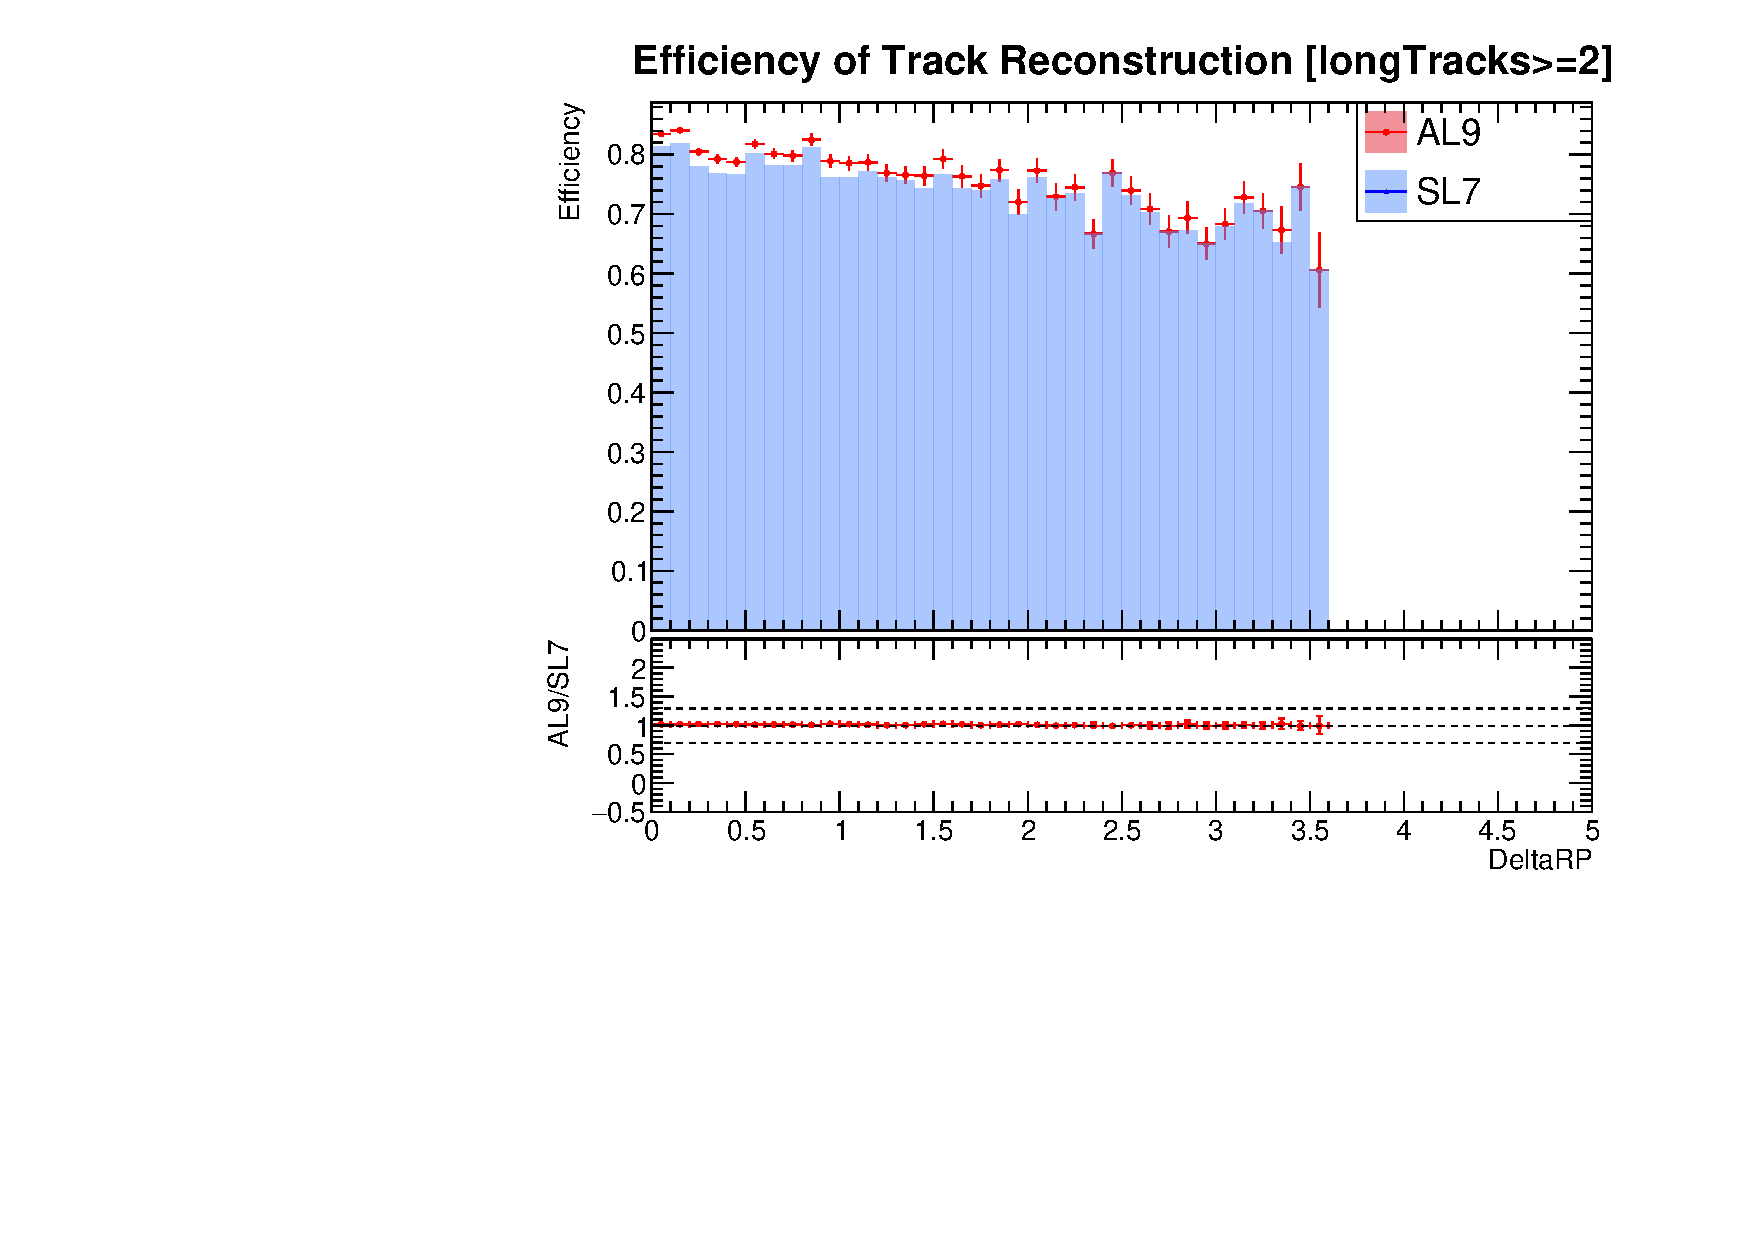
\includegraphics[width=\linewidth]{./output/Effi_greq2_DeltaRP.pdf}
    \end{figure}
\end{frame}

\begin{frame}{Comments on $>$2Track Efficiency}
    \begin{itemize}
        \item Good agreement between ALMA9 and CENTOS7
        \item Minor bump at very low separation ($\approx$ 2-6 mm) for ALMA9 
        \item Error Bars too significant to say anything about large separation
    \end{itemize}
\end{frame}

\begin{frame}{Alternate Efficiency Definition}
    \begin{itemize}
        \item Remove acceptance based on fiducial cuts at truth level
        \item Define Efficiency as the fraction of events with exactly 2 reconstructed longTracks divided by the total number of events. 
        \[ \text{Efficiency} = \frac{\text{NEvents}({= 2 \text{longTracks}})}{\text{NEvents}({\text{Total}})} \]
    \end{itemize}
\end{frame}

\begin{frame}{2 Track Efficiency as a function of DeltaR0}
    \begin{figure}
        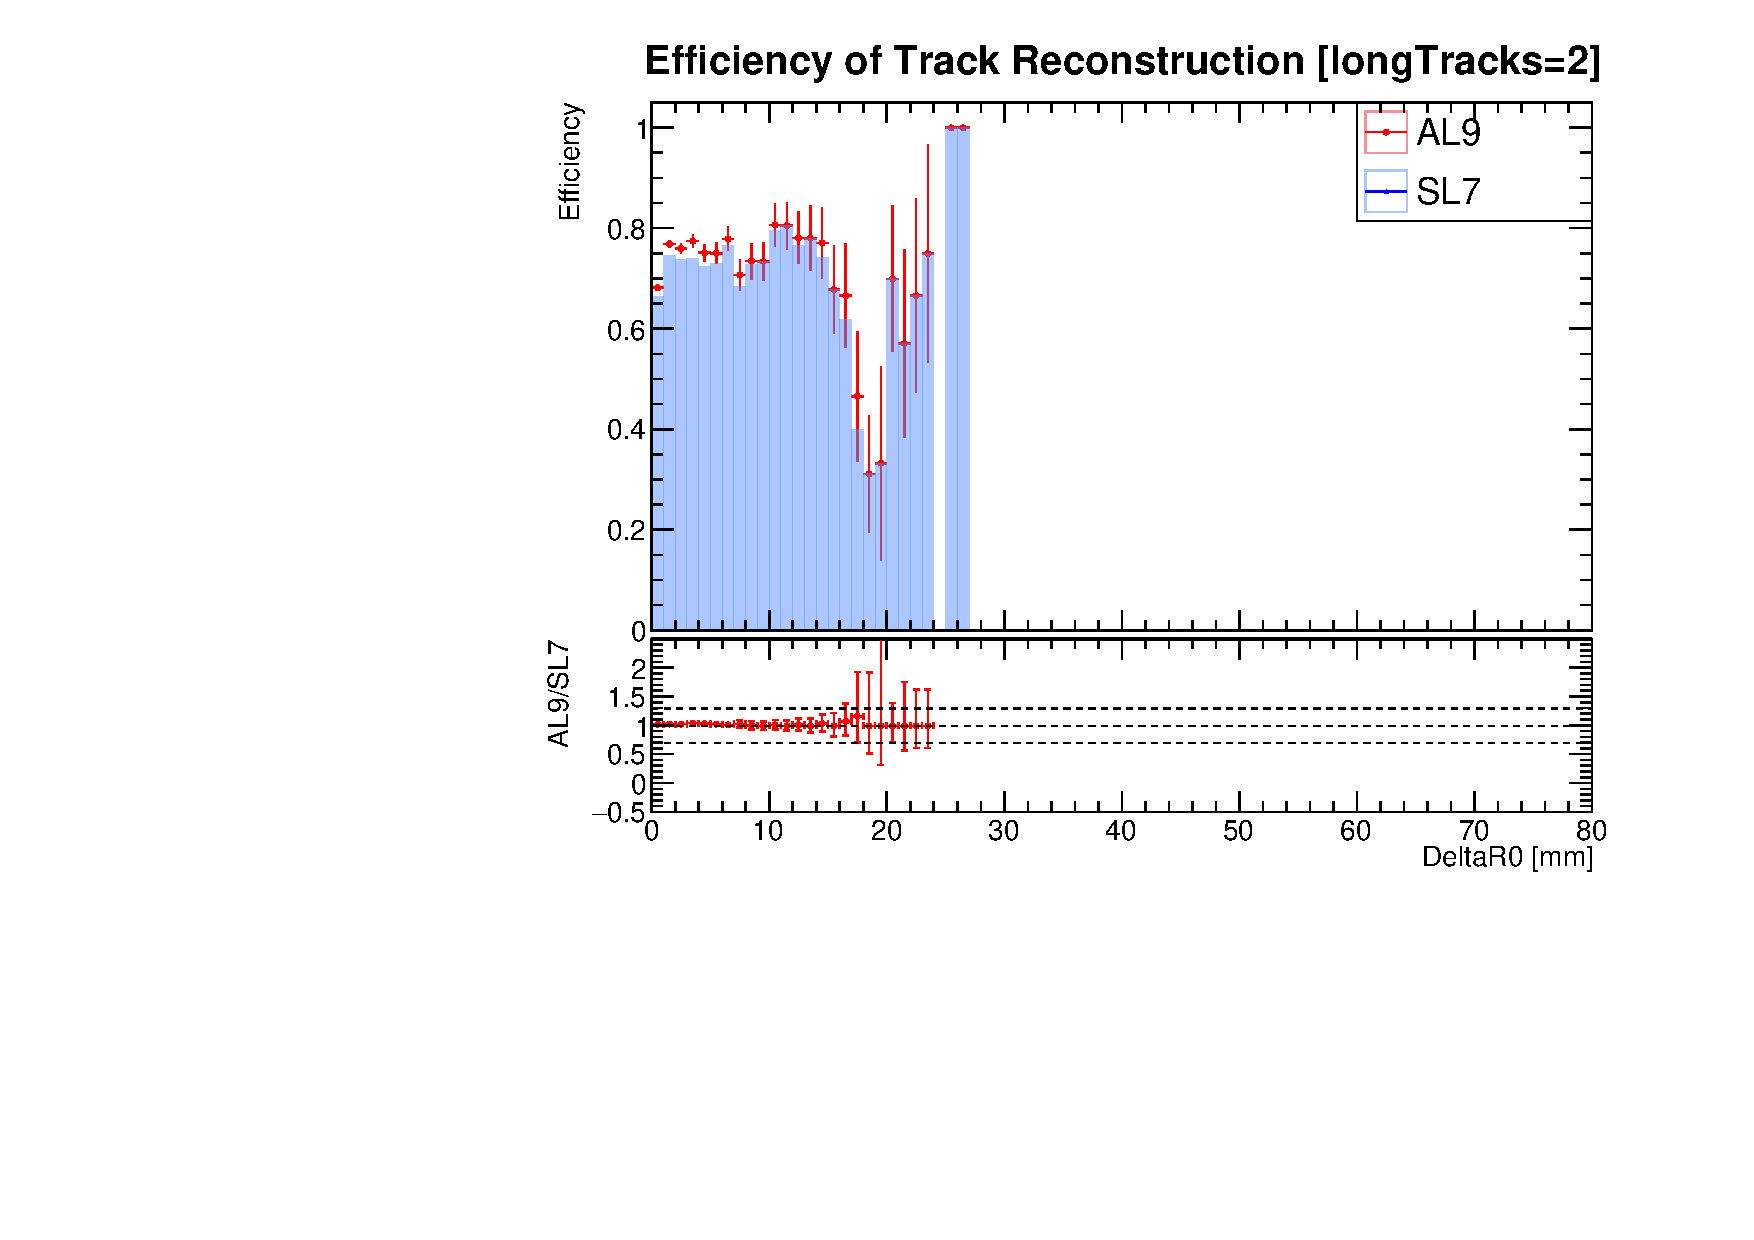
\includegraphics[width=\linewidth]{./output/Effi_eq2_DeltaR0.pdf}
    \end{figure}
\end{frame}
\begin{frame}{2 Track Efficiency as a function of DeltaX0 [SKIP]}
    \begin{figure}
        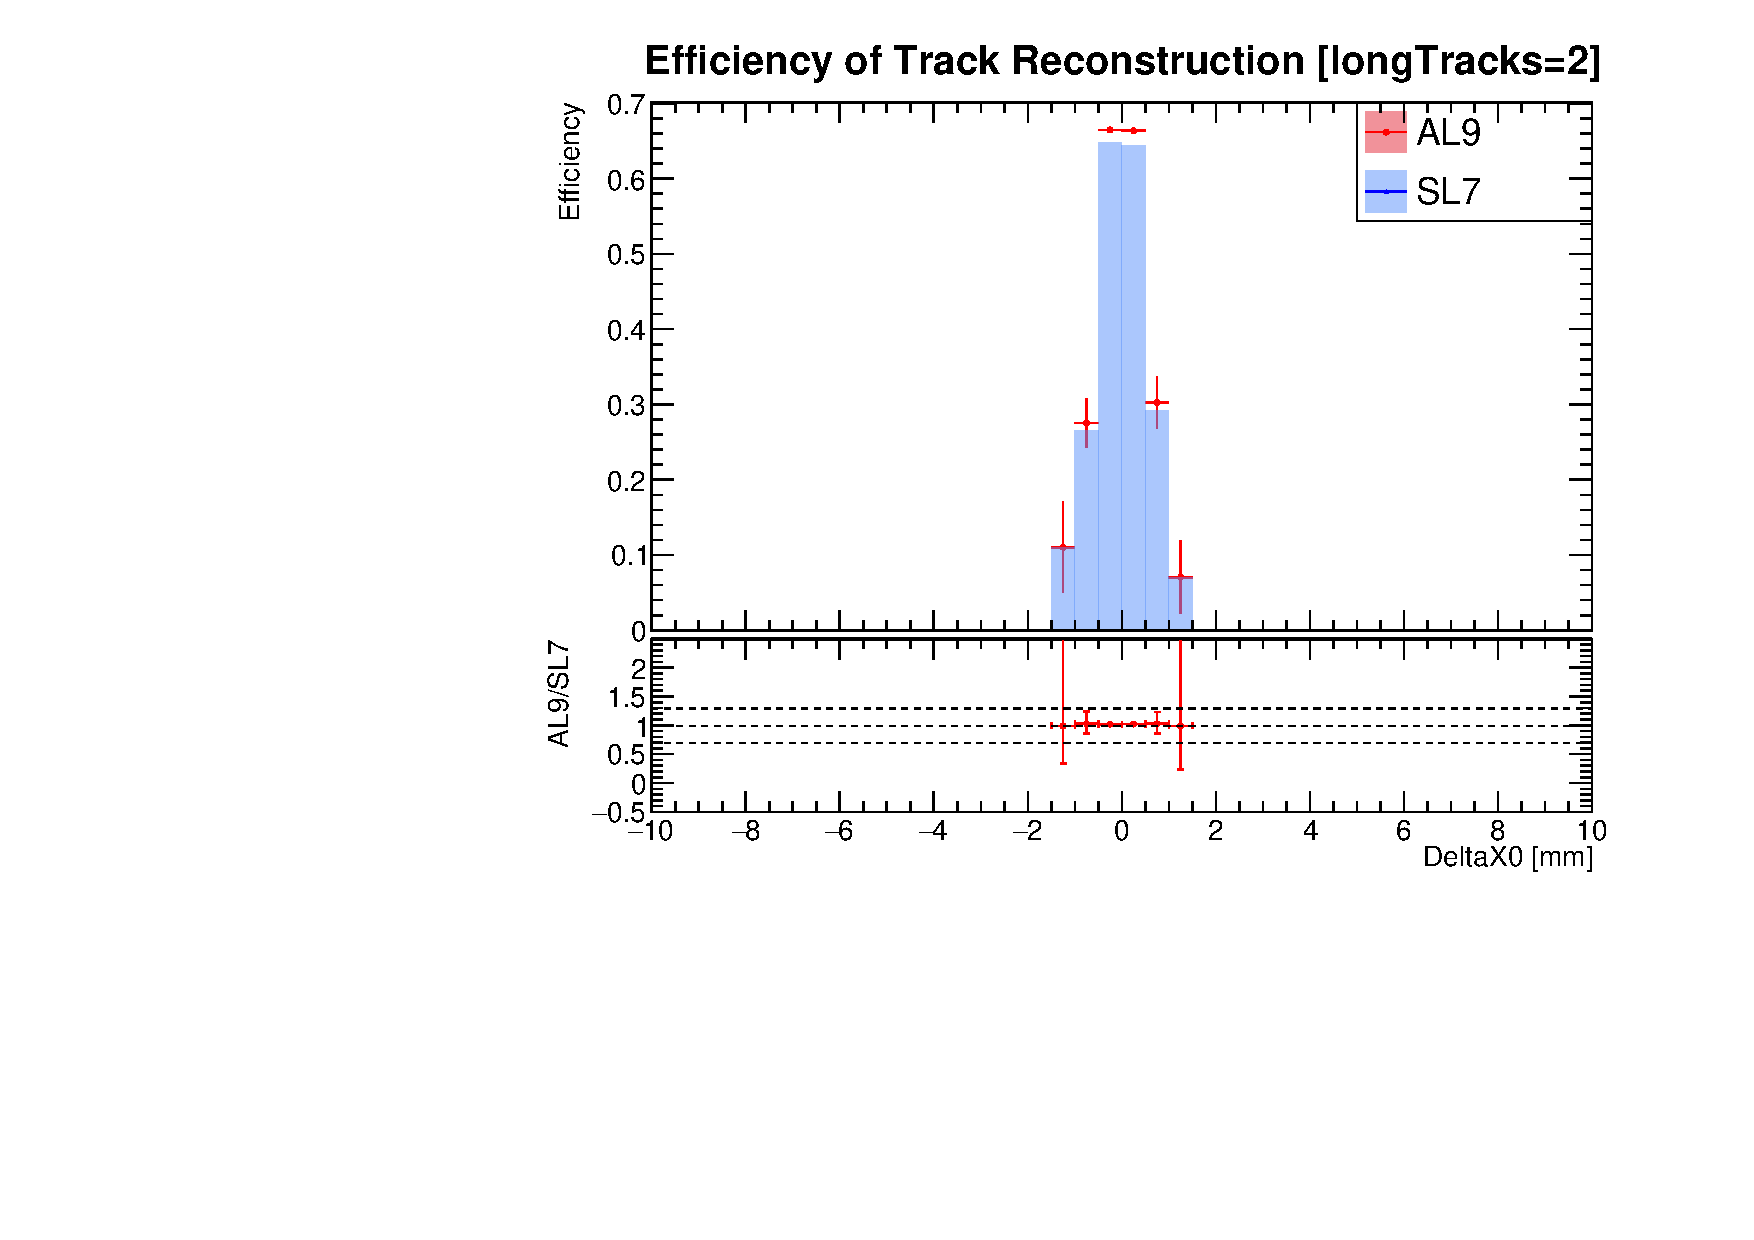
\includegraphics[width=\linewidth]{./output/Effi_eq2_DeltaX0.pdf}

    \end{figure}
\end{frame}
\begin{frame}{2 Track Efficiency as a function of DeltaY0 [SKIP]}
    \begin{figure}
        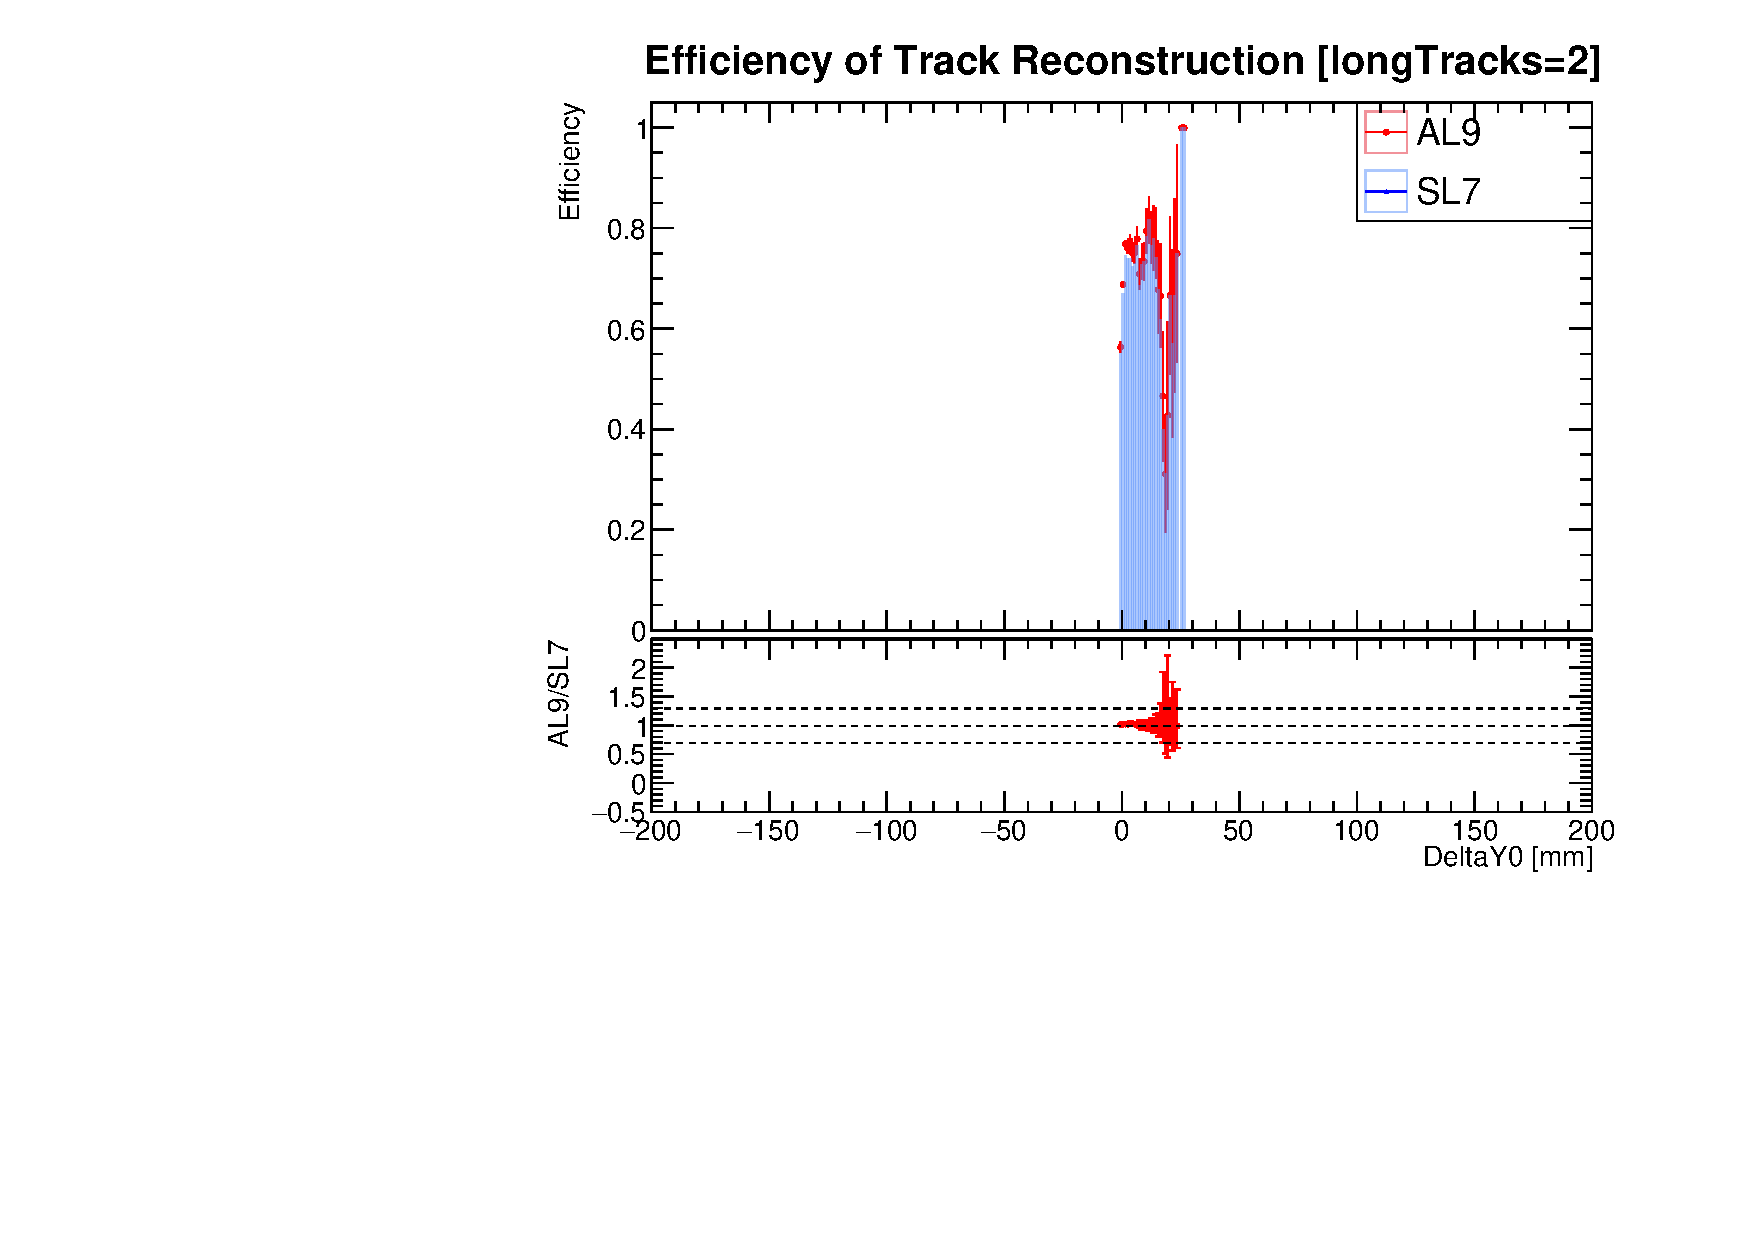
\includegraphics[width=\linewidth]{./output/Effi_eq2_DeltaY0.pdf}
    \end{figure}
\end{frame}
\begin{frame}{2 Track Efficiency as a function of Theta0}
    \begin{figure}
        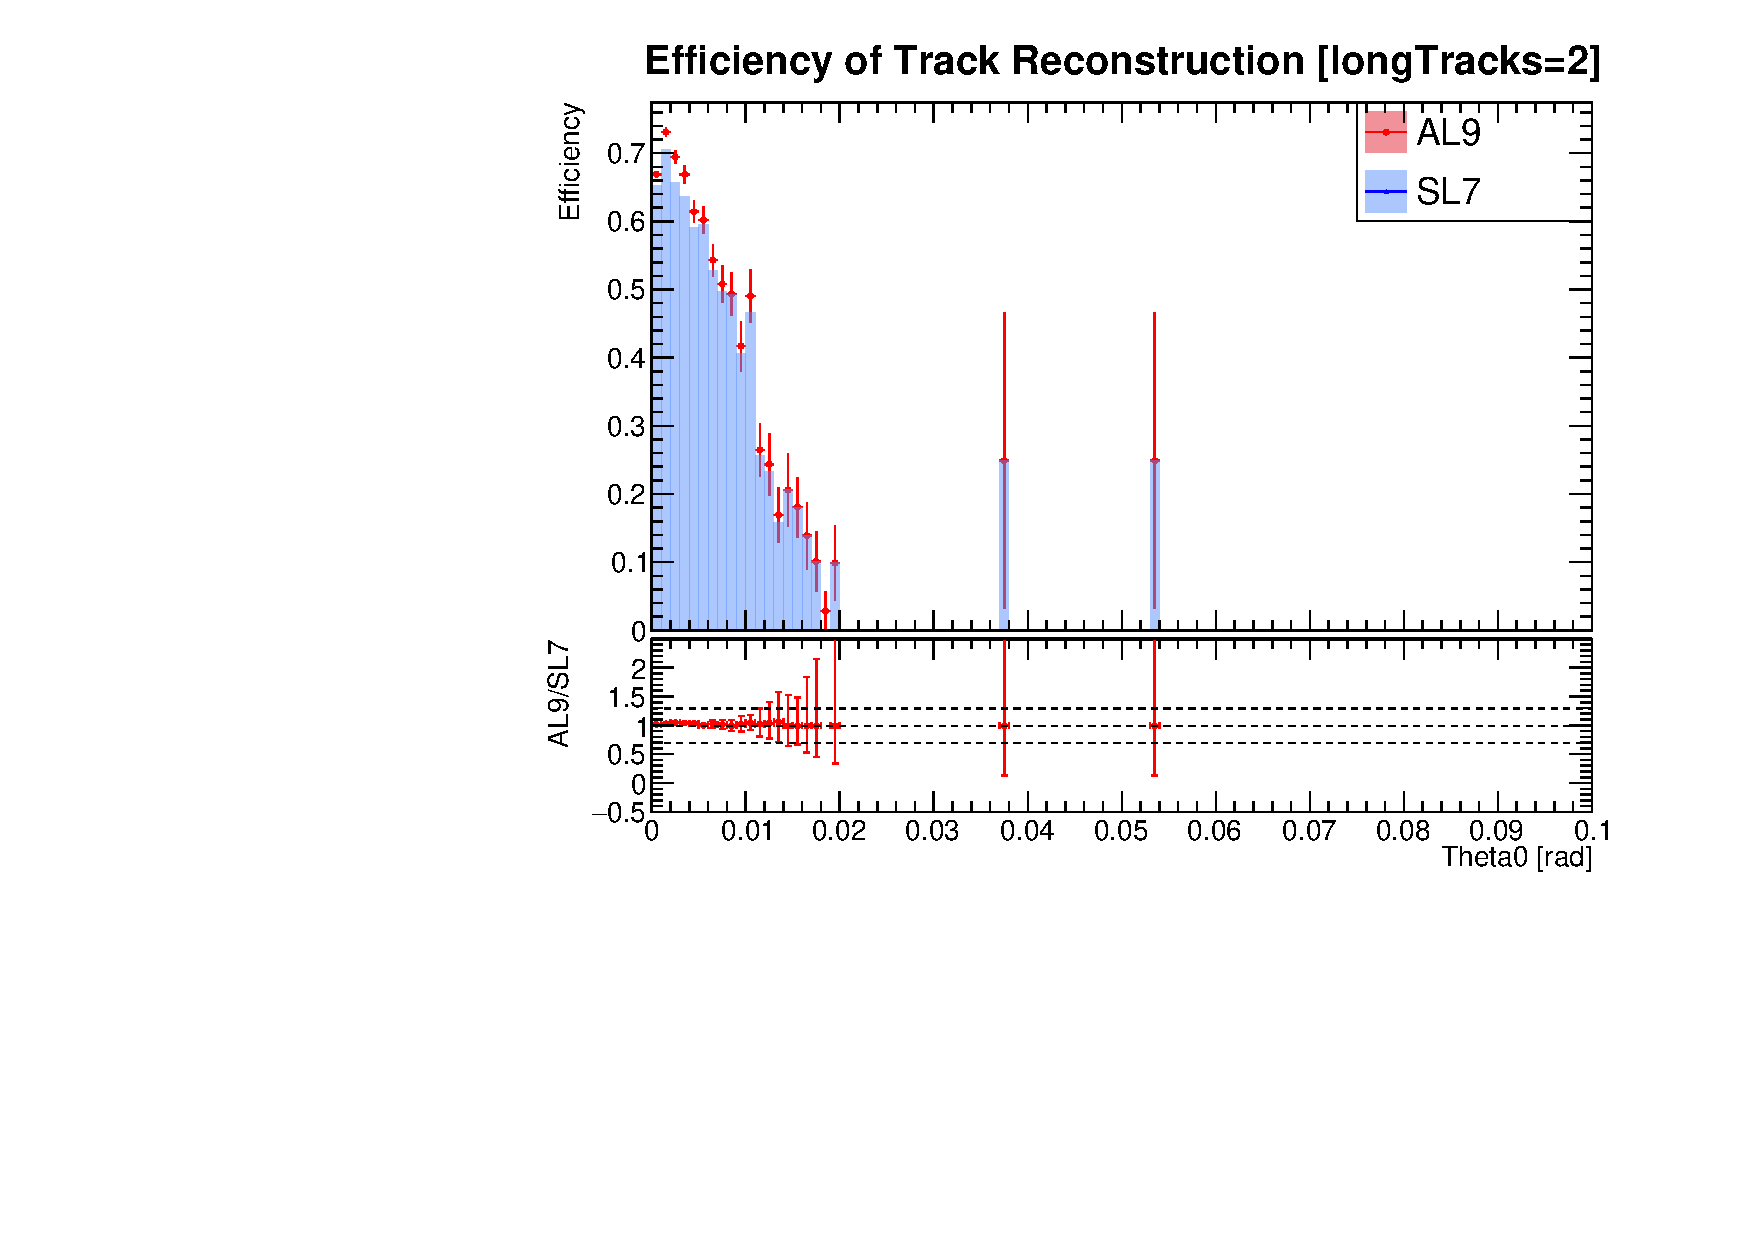
\includegraphics[width=\linewidth]{./output/Effi_eq2_Theta0.pdf}
    \end{figure}
\end{frame}
\begin{frame}{2 Track Efficiency as a function of DeltaRP}
    \begin{figure}
        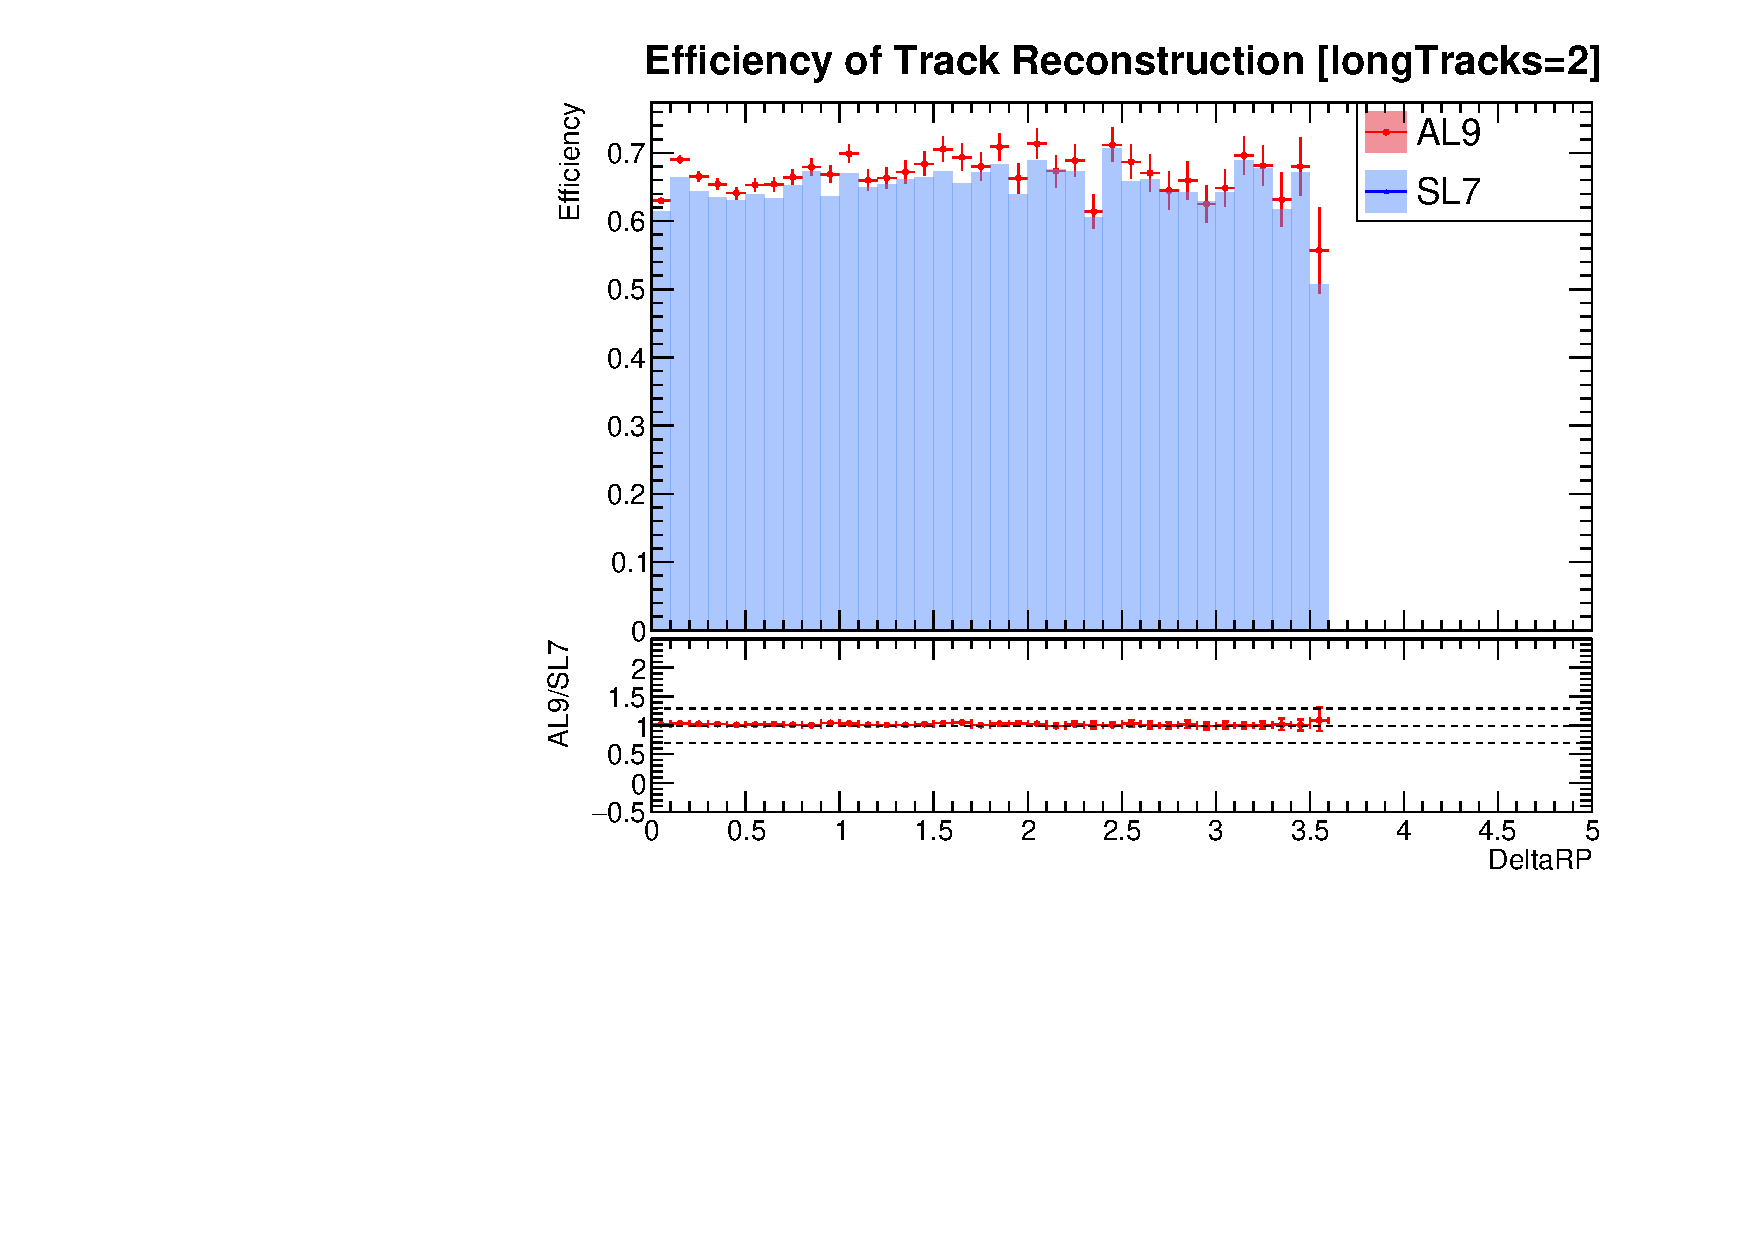
\includegraphics[width=\linewidth]{./output/Effi_eq2_DeltaRP.pdf}
    \end{figure}
\end{frame}

\begin{frame}{A More Robust Efficiency Metric [MC Based]}
    \begin{itemize}
        \item Our interest is only in the primary two tracks from $e^+e^-$
        \item For acceptance: Truth Position of $e^+e^-$ $<$ 100
        \item \text{\color{red}{\textbf{Identify the two primary tracks}} }
        \begin{itemize}
            \item Wanted to use t\_pdg\_parent \ldots
            \item Find closest to truth (by position and momenta)\dots 
            \item not trivial what is the margin of allowed error?
            \item Highest momenta tracks?
            \item Best approach is to use t\_truthHitRatio + PID
        \end{itemize}
        \item Can further quantify the ``goodness'' of the reconstructed primary tracks
    \end{itemize}
\end{frame}

\begin{frame}{Distribution of t\_pdg\_parent}
    \begin{table}[h!]
        \centering
        \small
        \begin{tabular}{|c|c|c|}
        \hline
        t\_pdg\_parent  & AL9       & SL7       \\ \hline
        -11             & 2         & 0         \\
        0               & 2         & 0         \\
        22              & 2610      & 2397      \\
        32              & 115877    & 112809    \\ \hline
        \end{tabular}
        \caption{Count of t\_pdg\_parent}
        \label{table:truth_efficiency}
        All particles are daughters of the Dark Photon? 
    \end{table}
    
\end{frame}

\section{Dark Photon CutFlow from Ansh's Study [SKIP]}
% \begin{frame}
    \includepdf[pages={3-5}]{assets/Alma9vsCentos7Efficiencies.pdf}
% \end{frame}

\begin{frame}{Comments on Data in NTuples [SKIP]}
    \begin{itemize}
        \item Need to add newly introducted variables to twiki.
        \item t\_st0\_x, y, z are filled with NaNs, We donot use/store station0 vals?
        \item t\_pdg\_parent ???
        \item truthParticleMatchedTracks - What exactly is this column.?
    \end{itemize}
    
\end{frame}